\chapter{Sprint 1 - Design and implementation}

\section*{Introduction}
\addcontentsline{toc}{section}{Introduction}
Previously, we detailed ERP Odoo and our project's progress. Now, we focus on Sprint 1, outlining its key objectives and functionalities.


\section{Sprint 1 Backlog}
The Sprint 1 Backlog lists product management tasks with their estimated durations for efficient planning.

Table \ref{tab:sprint1_product_management} details these tasks and durations..


\begin{longtable}{|c|p{8cm}|c|}
    \hline
    \rowcolor{purple!20} \textbf{N°} & \textbf{Tasks} & \textbf{Duration} \\ \hline
    \endfirsthead
    \hline
    \rowcolor{purple!20} \textbf{N°} & \textbf{Tasks} & \textbf{Duration} \\ \hline
    \endhead
    1 & - As an administrator, I can manage products in the system. & 7 Days \\ \hline
    2 & - As an administrator, I can add new products. & 2 Day \\ \hline
    3 & - As an administrator, I can update existing product details. & 2 Days \\ \hline
    4 & - As an administrator, I can delete outdated products. & 2 Day \\ \hline
    5 & - As an administrator, I can manage periods. & 6 Days \\ \hline
    6 & - As an administrator, I can manage the rental pricing. & 4 Days \\ \hline
    \caption{Sprint 1 Backlog for Product Management}
    \label{tab:sprint1_product_management}
\end{longtable}

\section{Functional Specifications}

\subsection{Use Case Diagram}

In this section, we present the functional specifications for the Product Management module.\\

\begin{figure}[h]
    \centering
    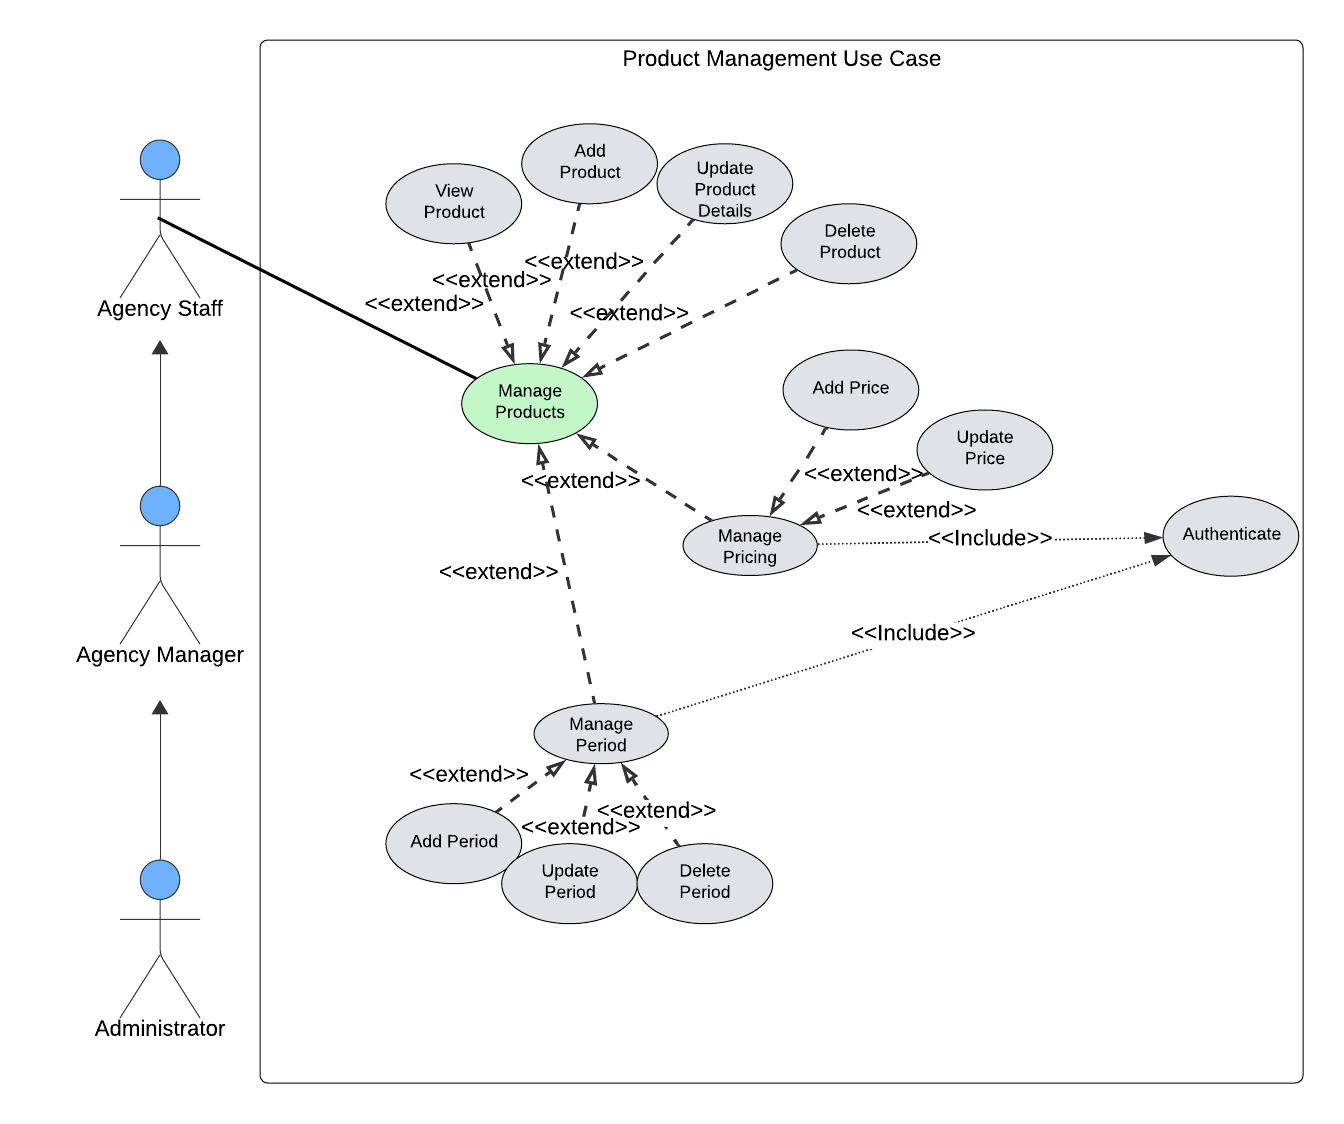
\includegraphics[width=1\textwidth]{sprint1/sprint1usecase.png}
    \caption{Sequence Diagram for "Product Management"}
    \label{fig:product_management_use_case}
\end{figure}

\subsection{Sequence Diagram}
The Sequence Diagram \cite{sequencediagram} illustrates how objects interact to add a new product in Sprint 1, detailing message exchanges and data flow.

\begin{itemize}
    \item Administrator requests new product creation, triggering a form.
    \item Administrator submits form, system verifies data.
    \item Valid data prompts addition to database.
    \item System confirms and displays read-mode form.
    \item Invalid data keeps form in read mode for corrections.
\end{itemize}

\begin{figure}[h]
    \centering
    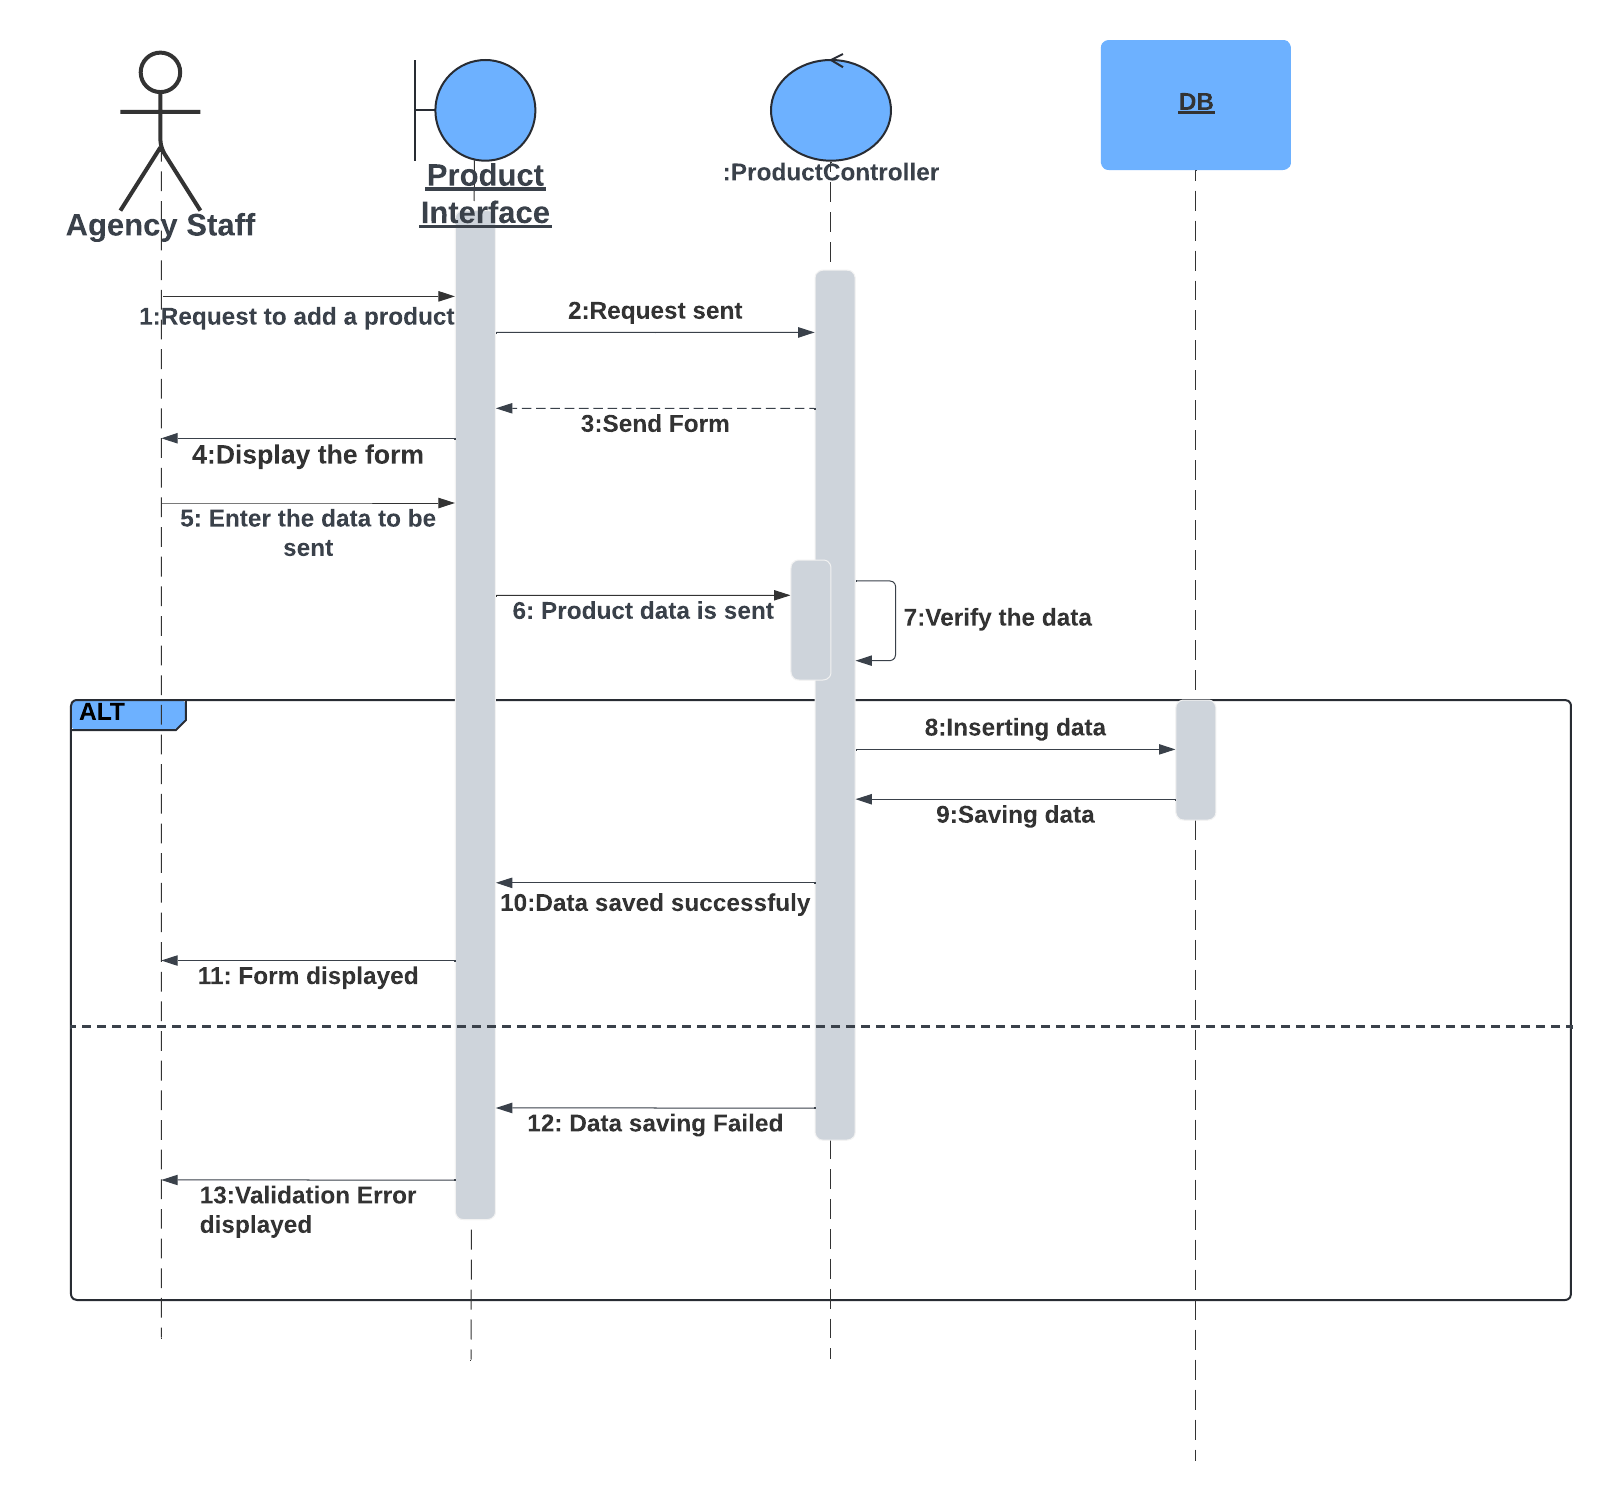
\includegraphics[width=0.9\textwidth]{sprint1/Sprint1Sequence.png}
    \caption{Sequence Diagram for "Product Management"}
    \label{fig:product_management_sequence_diagram}
\end{figure}
\newpage
\section{Sprint Realization}

\subsection{Login Process for Agency Staff in Odoo}
\begin{itemize}
    \item Agency staff authenticate by entering their credentials.
    \item System verifies submitted username and password.
    \item Valid credentials grant access; invalid ones prompt re-entry.
\end{itemize}

\begin{figure}[h]
    \centering
    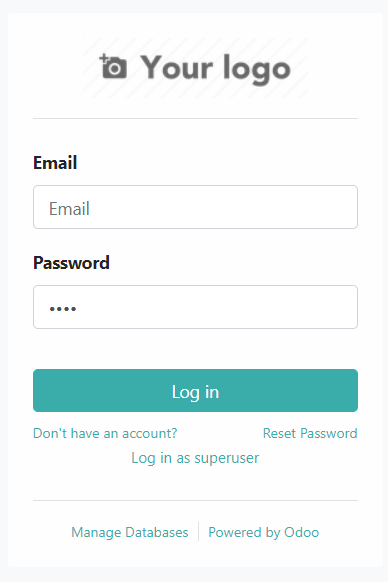
\includegraphics[width=0.45\textwidth]{sprint1/login.png}
    \hfill
    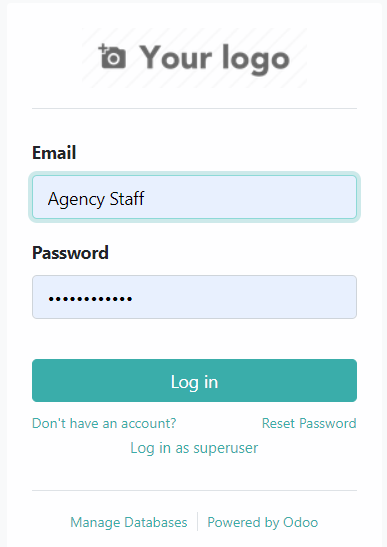
\includegraphics[width=0.45\textwidth]{sprint1/login2.png}
    \caption{Login Process for Agency Staff}
    \label{fig:login_process}
\end{figure}



\section{Product Interface}

\subsection{General Information Notebook}
The "General Information" notebook contains essential details about the product, such as name, type, and category, providing foundational information for product management.
\begin{figure}[!h]
    \centering
    \makebox[\textwidth][c]{%
        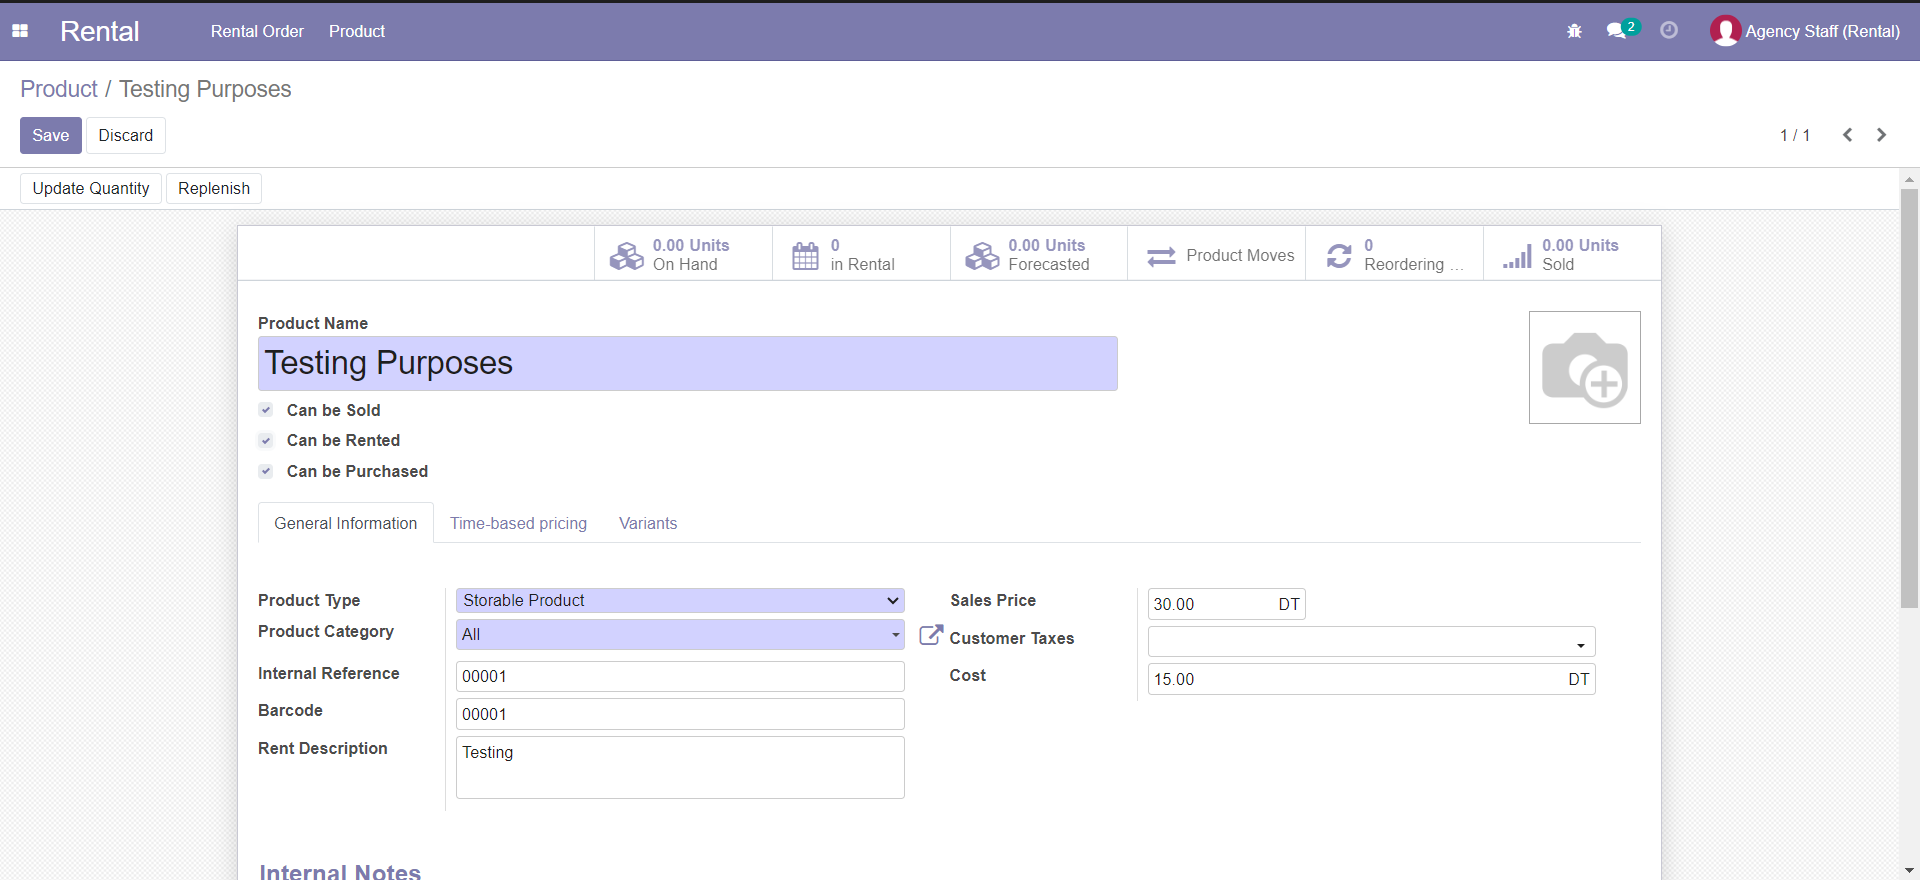
\includegraphics[width=1.2\textwidth]{sprint1/product1.png}} % replace with your image path
    \caption{General Information Notebook}
    \label{fig:general_information}
\end{figure}
\newpage

\subsection{Time-Based Pricing Notebook}
The "Time-Based Pricing" notebook is designed for rental products, allowing users to configure pricing based on different rental periods, such as hourly, daily, or weekly rates.
\begin{figure}[h]
    \centering
    \makebox[\textwidth][c]{%
        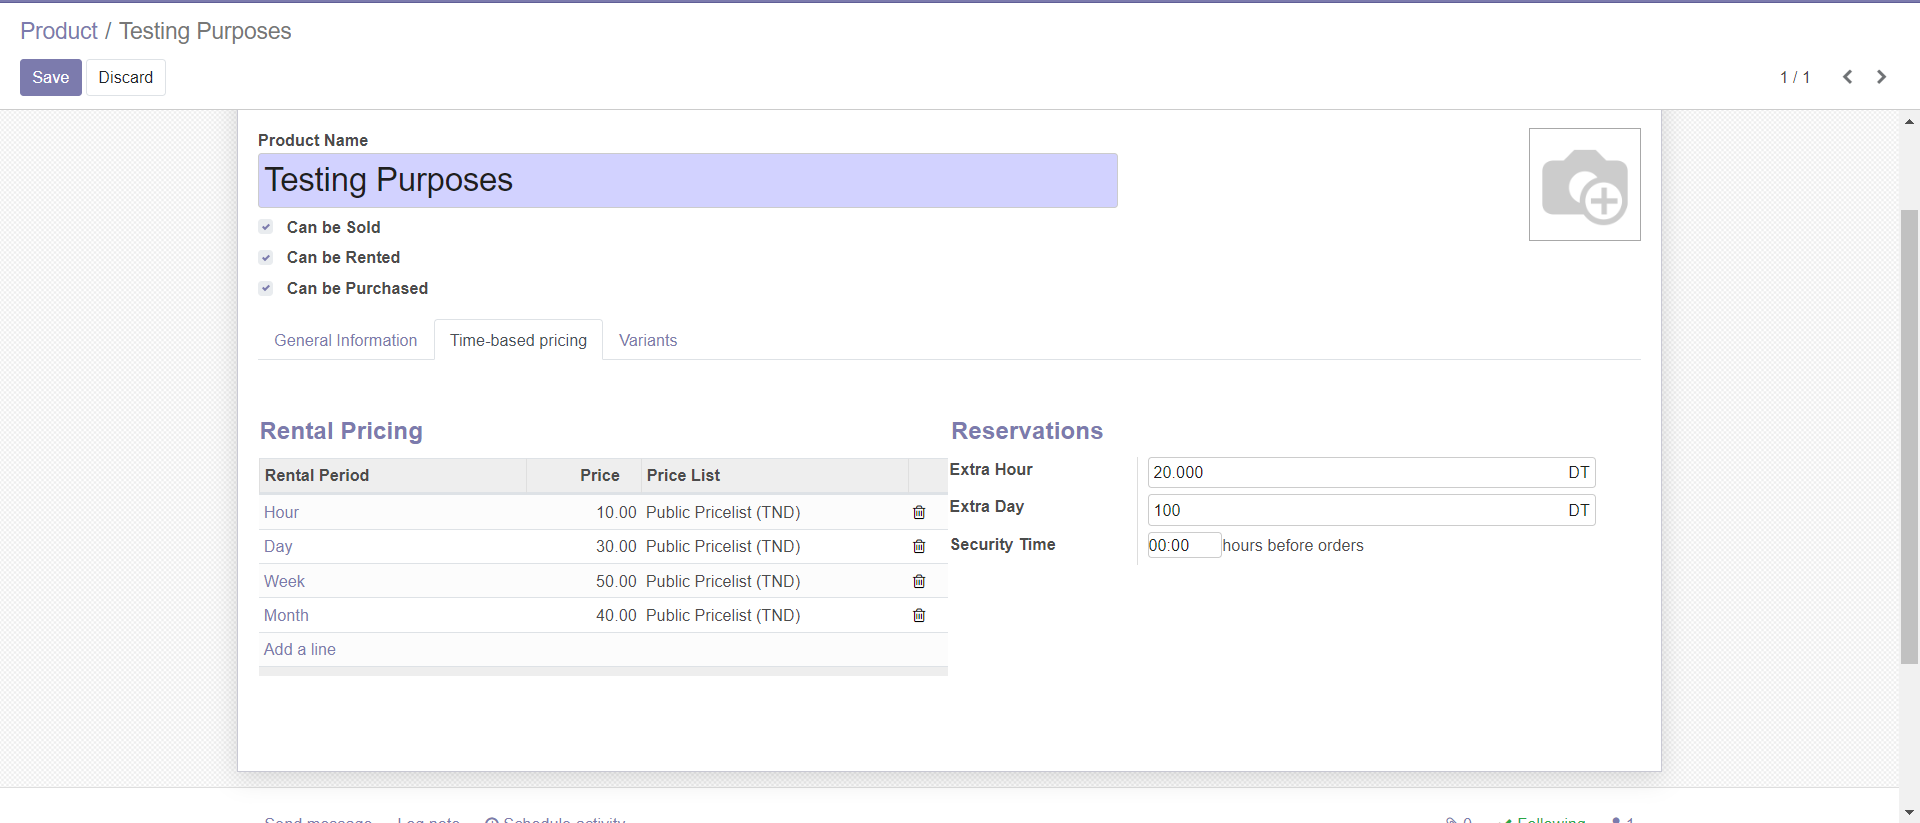
\includegraphics[width=1.2\textwidth]{sprint1/product2.png}} % replace with your image path
    \caption{Time-Based Pricing Notebook}
    \label{fig:time_based_pricing}
\end{figure}

\subsection{Variants Notebook}
The "Variants" notebook manages product variants, enabling the creation and editing of different versions of a product with various attributes like size and color, ensuring accurate representation and pricing within the product catalog.
\begin{figure}[h]
    \centering
    \makebox[\textwidth][c]{%
        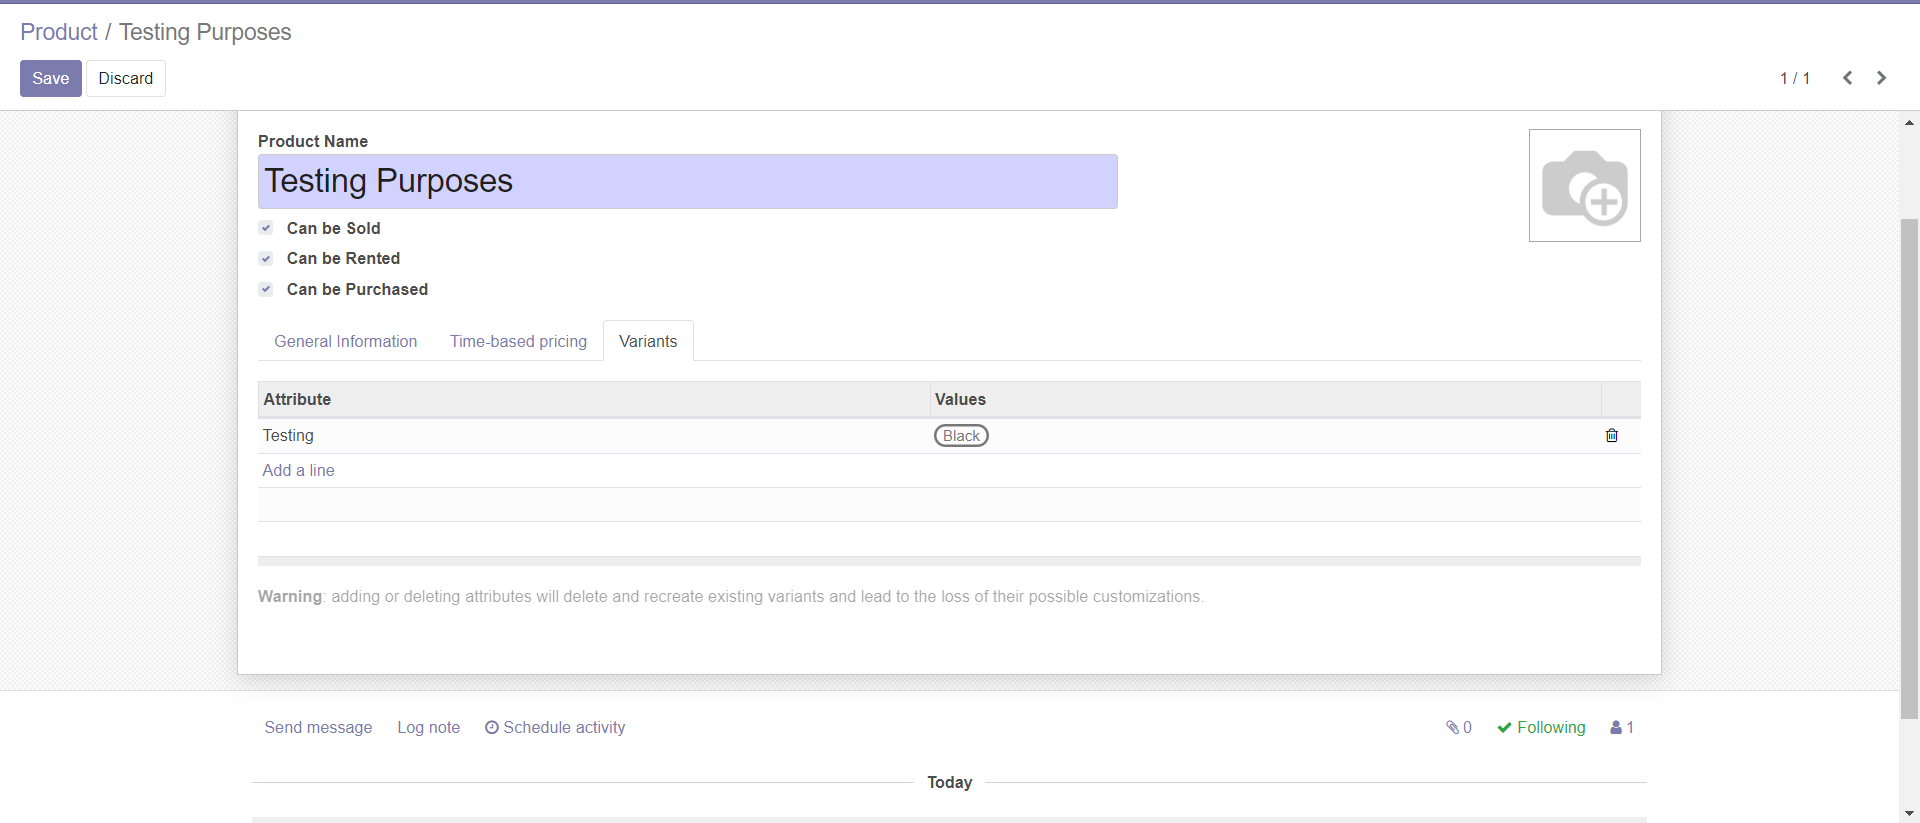
\includegraphics[width=1.2\textwidth]{sprint1/product3.png}} % replace with your image path
    \caption{Variants Notebook}
    \label{fig:variants}
\end{figure}

\subsection{Update Quantity Button}
The "Update Quantity" button allows administrators to manually adjust the stock levels of a product, ensuring inventory accuracy by reflecting real-time changes in stock quantities.
\begin{figure}[h]
    \centering
    \makebox[\textwidth][c]{%
        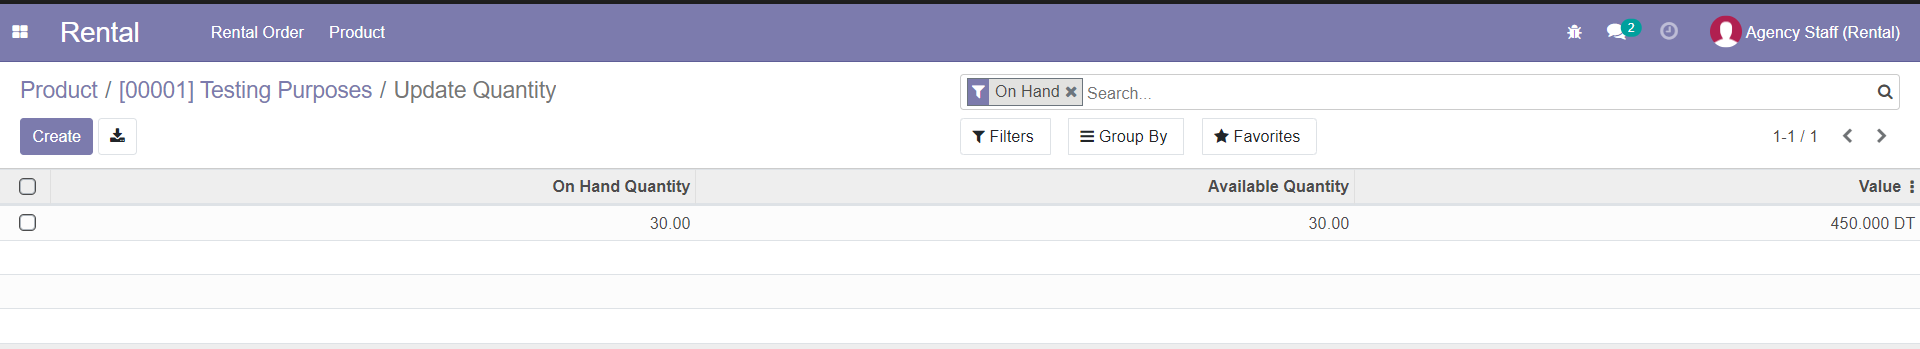
\includegraphics[width=1.2\textwidth]{sprint1/product4.png}} % replace with your image path
    \caption{Update Quantity Button}
    \label{fig:update_quantity}
\end{figure}

\subsection{Quantity on Hand Display}
After updating the quantity, the "Quantity on Hand" display reflects the new stock levels, providing an accurate overview of available inventory to help in managing stock efficiently.
\begin{figure}[h]
    \centering
    \makebox[\textwidth][c]{%
        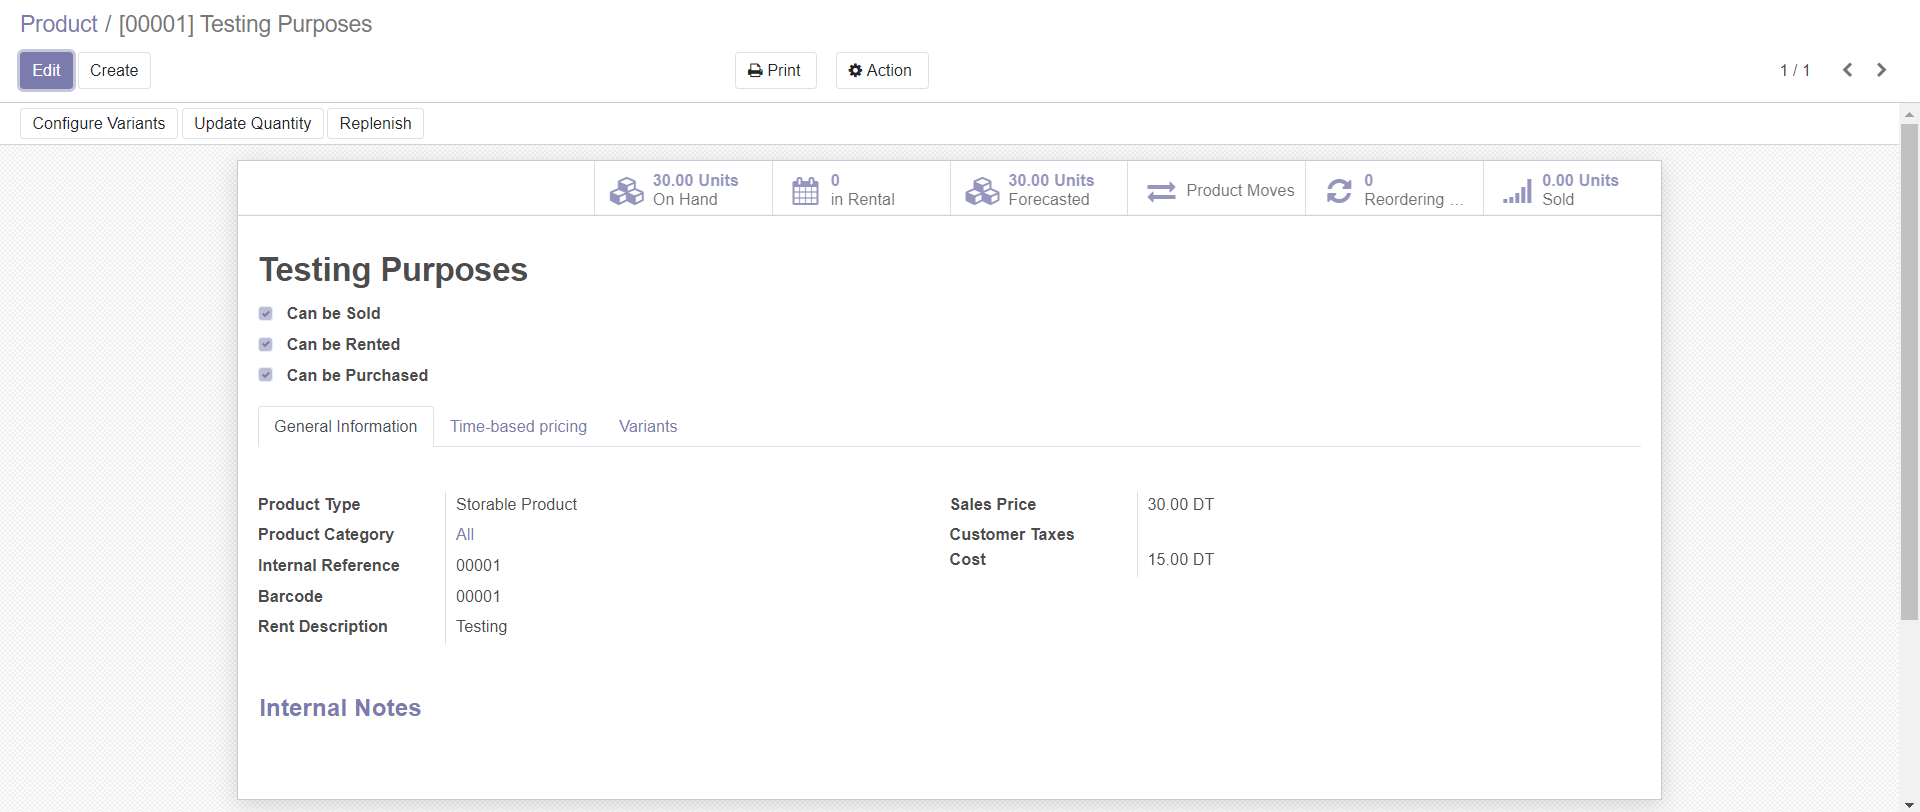
\includegraphics[width=1.2\textwidth]{sprint1/product5.png}} % replace with your image path
    \caption{Quantity on Hand Display}
    \label{fig:quantity_on_hand}
\end{figure}

\section*{Conclusion}
\addcontentsline{toc}{section}{Conclusion}
In Sprint 1, we established key functionalities in the product management module of Odoo ERP. This included "General Information," "Time-Based Pricing," and "Variants" notebooks, along with the "Update Quantity" button and "Quantity on Hand" display, enhancing product management and inventory accuracy.

In the next sprint, we will focus on the rental order process, including reservations, rental stock tracking, to further support rental operations.